% 按固定答案扫描页9图4-5-8的可见关系重绘；含平面内投影点D，仅作示意、不按比例。
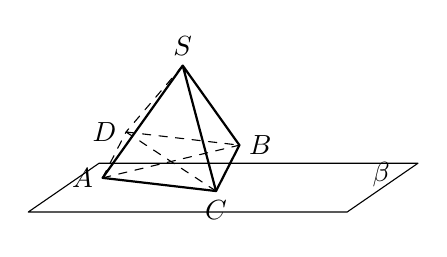
\begin{tikzpicture}[x=0.9cm,y=0.62cm,line cap=round,line join=round]
  \coordinate (P1) at (-2.5,-0.85);
  \coordinate (P2) at (2.0,-0.85);
  \coordinate (P3) at (3.0,0.15);
  \coordinate (P4) at (-1.5,0.15);
  \coordinate (A) at (-1.45,-0.15);
  \coordinate (C) at (0.15,-0.42);
  \coordinate (B) at (0.48,0.52);
  \coordinate (D) at (-1.12,0.79);
  \coordinate (S) at (-0.32,2.15);

  \draw[thin] (P1)--(P2)--(P3)--(P4)--cycle;
  \node at (2.48,-0.08) {$\beta$};

  \draw[thick] (A)--(C)--(B);
  \draw[dashed] (A)--(B);
  \draw[thick] (S)--(A) (S)--(B) (S)--(C);
  \draw[dashed] (S)--(D) (A)--(D) (D)--(B) (C)--(D);

  \node[left] at (A) {$A$};
  \node[below] at (C) {$C$};
  \node[right] at (B) {$B$};
  \node[left] at (D) {$D$};
  \node[above] at (S) {$S$};
\end{tikzpicture}
